\documentclass{article}
\usepackage[icelandic]{babel}
\usepackage[T1]{fontenc}
\usepackage[utf8]{inputenc}

\usepackage{graphicx}
\usepackage{wrapfig}
\usepackage{float}

\begin{document}

\tableofcontents
\newpage

\section{Inngangur}

\newpage

\section{Sprettir}
Verkefnið okkar var þannig lagt upp af DataMarket, að þeir vildu í fyrsta lagi fá heilstætt kerfi sem skilaði niðurstöðum. 
Þær niðurstöður þyrftu þó ekki að verja mjög marktækar og byggja á flóknum reikniaðferðum. Því næst áttum við að þróa reikniaðferðirnar eins 
mikið og mögulegt væri, á þeim tíma sem við höfðum. Þetta verkefni var því mjög opið og ljóst að mikilvægt væri 
af okkar hálfu að halda góðri yfirsýn allan tímann, svo að ekki yrði farið lengra í bætingum en svo að það myndi nást að fullklára þær 
aðferðir sem við ætluðum að hafa í kerfinu, í tæka tíð. Því lögðum við upp með að vinna verkið í tveimur fösum. Áætlunin var þannig að skipuleggja
einungis fyrri fasan í upphafi. Byrja að kynna okkur meðfram þeim fasa hvað við gætum mögulega gert í seinni fasanum, en taka ekki ákvarðanir 
um hvað yrði gert fyrr en í upphafi seinnifasa.

\subsection{Sprettur 0}
Sprettur 0 var settur upp sem undirbúnings sprettur. Ekki voru sögur eins og í hefbundnum spretti, heldur notuðum við þennan tíma til að 
skipuleggja verkáætlun, gerðum áhættugreiningu og unnum að ýmsum öðrum undirbúiningi.
\subsection{Sprettur 1}
Í fyrsta spretti fórum við í að kynna okkur tæknileg atriði sem við ætluðum að nota.
Flest þekktum við, en höfðum ekki unnið með það í Python áður. Þetta voru hlutir eins og prófandrifin þróun, REST-ful þróun og hvernig 
unnið er með JSON skrár. Einnig settum við upp grunn að kerfinu sem gat sótt gögn frá DataMarket. Náðum ekki alveg að kára það sem við lögðum 
upp með og urðum að færa hluta úr sögum yfir í næsta sprett.
\begin{figure}[H]
  \centering
  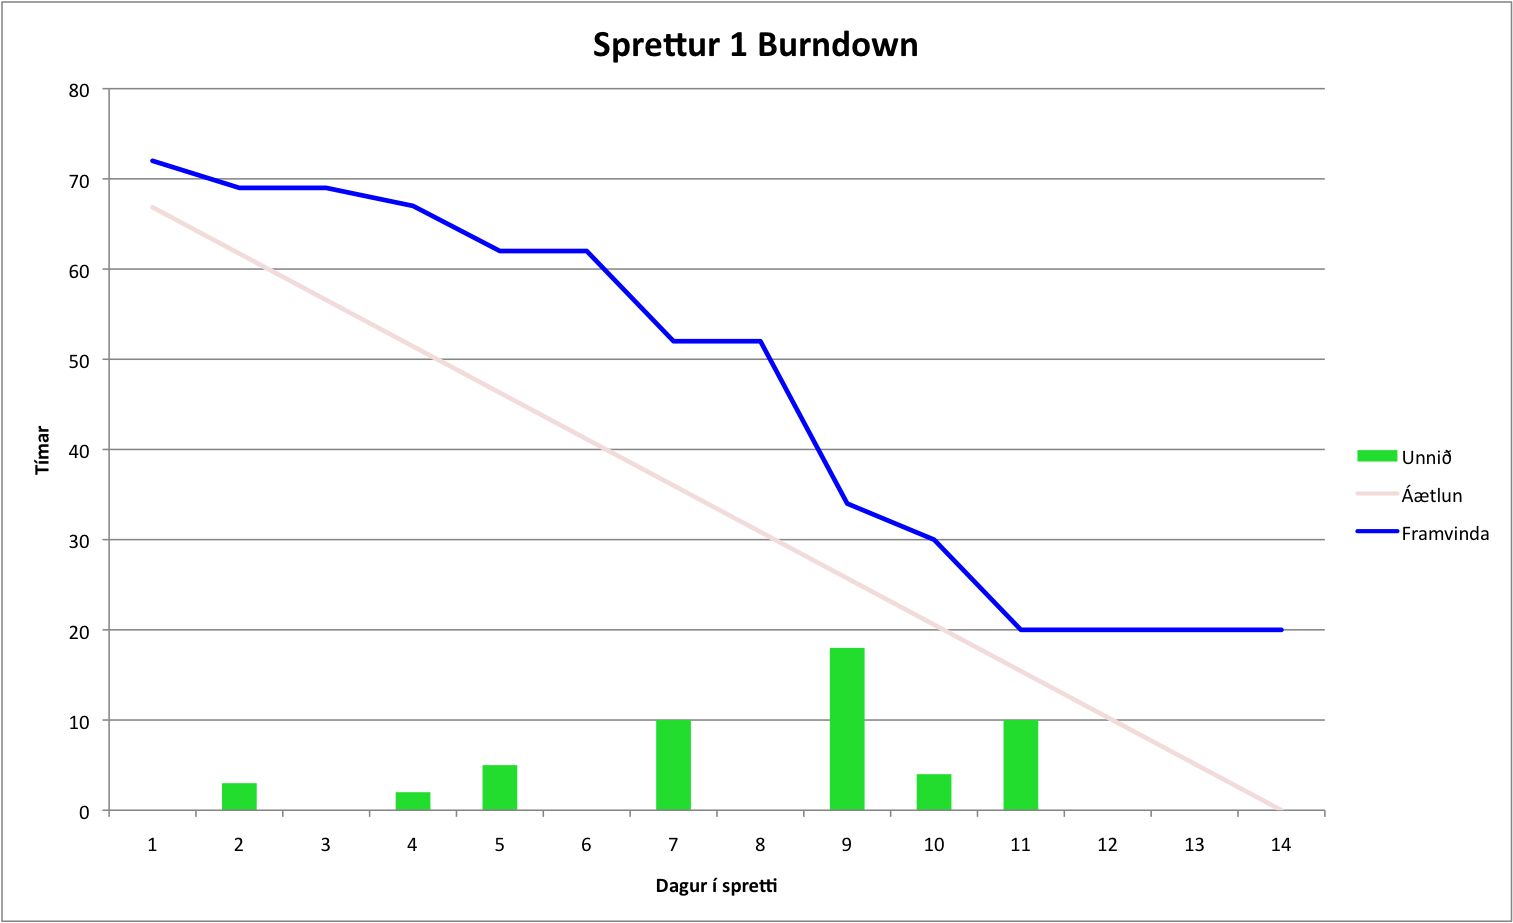
\includegraphics[width=0.72\textwidth]{Sprettur1_Burndown.png}
  \caption{Sprettur 1 Burndown}
\end{figure}

\subsection{Sprettur 2}
Í spretti 2 fundum við áhugaverð gögn hjá Datamarket settum upp staðbunda gátt(e.service stub),svo að það myndi ekki hindra okkur í þróun ef 
aðgangur að gagnagrunni Datamarket væri ekki til staðar. Þetta var hluti af okkar áhættugreiningu (VÍSUN í KAFLA). 
Þá bjugum við til fyrstu reikniaðferðirnar, meðaltal miðgildi og staðalfrávik, og létum kerfið sækja gögn og skila niðurstöðum.
Þá áttum við fundi með sérfræðingum á sviði stærðfræði og tölfræði, til að ýta úr vör hugmyndavinnu fyrir seinni fasa.
\begin{figure}[H]
 \centering
 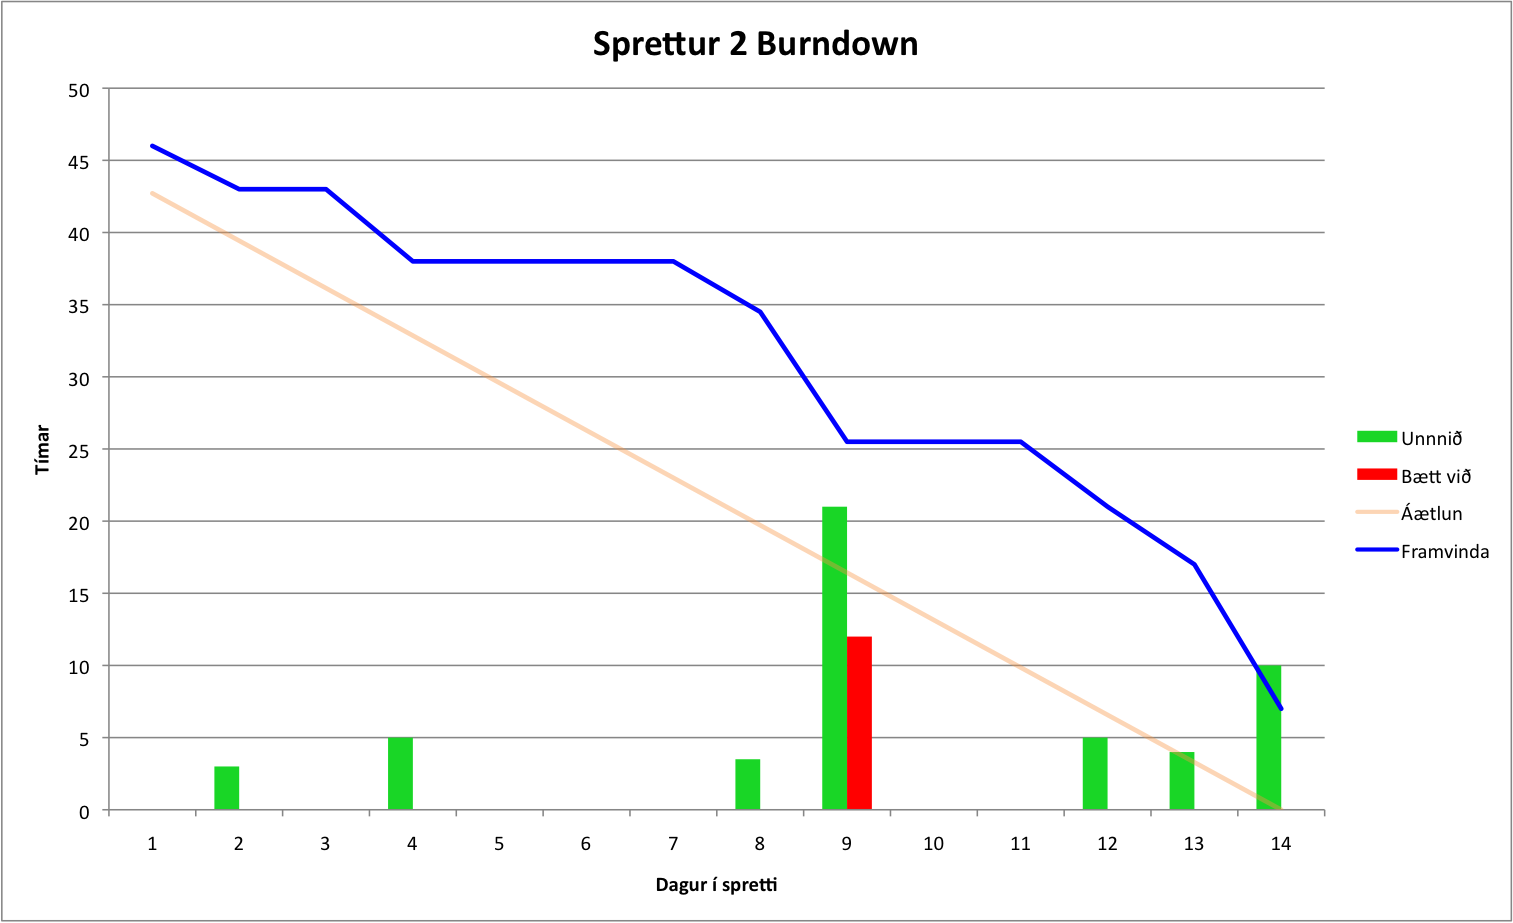
\includegraphics[width=0.72\textwidth]{Sprettur2_Burndown.png}
 \caption{Sprettur 2 Burndown}
\end{figure}
\subsection{Sprettur 3}
Þegar hér var komið við sögu vorum við farnir að finna ákveðinn takt í áætlanagerð og sáum betur hvað við gátum gert ráð fyrir að klára mikið 
í einum sprett. Setum upp aðgerðarsöfn(e. libraries) sem voru til þess fallin að aðstoða okkur við útreikninga. Það tók þó umtalsvert meiri tíma en við gerðum
ráð fyrir. Þá bættum við staðbundnu gáttina og kynntum okkur aðgerðarsöfnin.
\begin{figure}[H]
 \centering
 \includegraphics[width=0.72\textwidth]{Sprettur3Burndown.png}
 \caption{Sprettur 3 Burndown}
\end{figure}
\subsection{Sprettur 4}
Spretturinn fór í að setja upp framenda á kerfið og forma skýrsluna sem það skilar af sér. Þegar við vorum svo farnir að nota aðgerðarsöfnin 
kom á daginn að einföldu aðferðirnar okkar voru mun betri en vonir stóðu til. Einnig komumst við að því að það hafa aðrir beitt þessum aðferðum 
og kallast þær Bollinger bönd ( SJÁ KAFLA UM BOLLINGER BÖND ). 

Við gátum nú sýnt þeim hjá Datamarket niðurstöður úr kerfinu okkar og við það urðu til fleiri hugmyndir um hvernig hægt væri að nýta það ( SJÁ LÝSING VERKEFNIS ).

\begin{figure}[H]
 \centering
 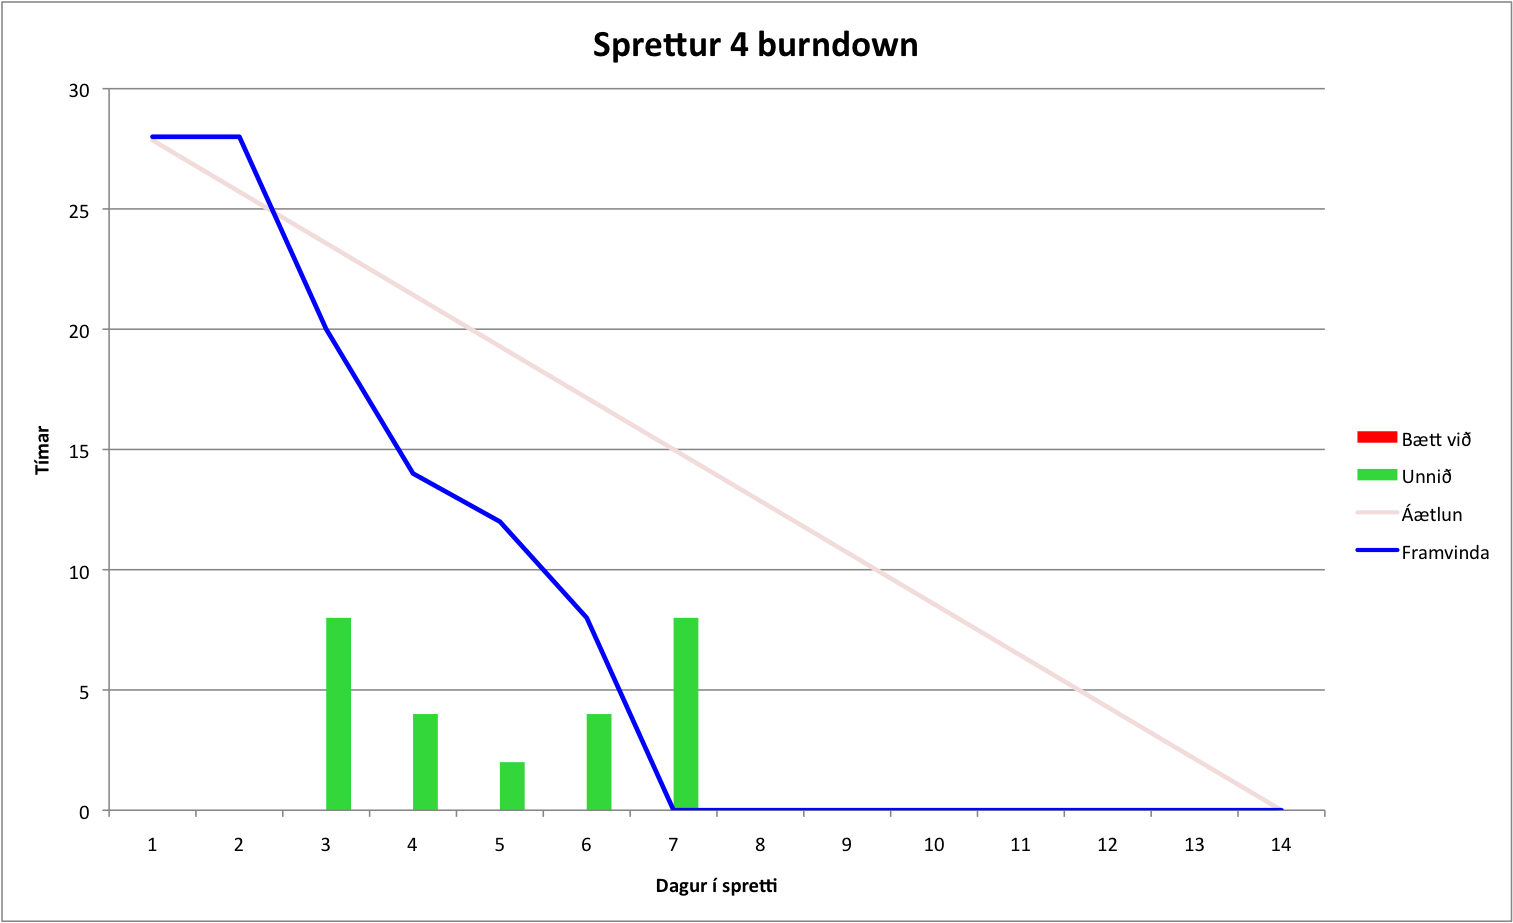
\includegraphics[width=0.72\textwidth]{Sprettur4_Burndown.png}
 \caption{Sprettur 4 Burndown}
\end{figure}

\subsection{Sprettur 5}
Síðasti sprettur í fasa 1. Funduðum með DataMarket og ákváðum endanlegt form á flöggum sem er skilað. Gengum frá lausum endum, og kóði yfirfarinn 
(e. refactor) og útgáfa 1.0 varð til. Hugmyndavinna fyrir fasa 2 komin á fullt.

\begin{figure}[H]
 \centering
 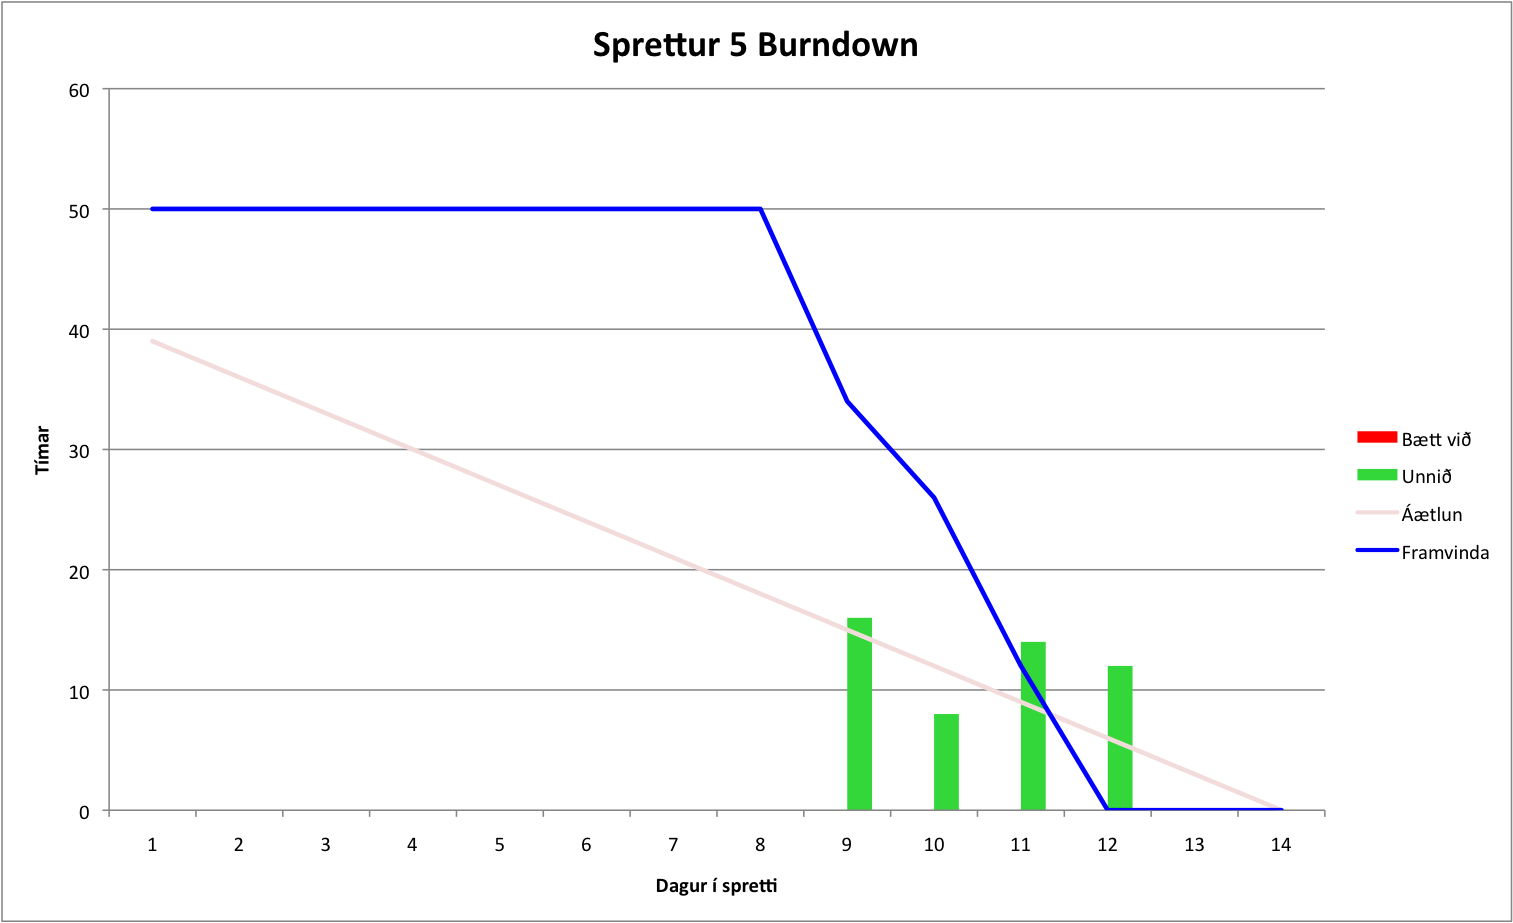
\includegraphics[width=0.72\textwidth]{Sprettur5_Burndown.png}
 \caption{Sprettur 5 Burndown}
\end{figure}

\subsection{Sprettur 6}
Við höfðum sankað að okkur mikið af upplýsingum og höfðum ákveðnar hugmyndir um hvað okkur langaði að gera. Það krafðist þess hinsvegar að við 
þurftum að framkvæma prófanir til að sjá hvað myndi henta okkar kerfi best. Því skipulögðum við sprettinn létt og bættum í hann þegar líða tók á. 
Fljótlega komumst við þó að niðurstöðum um hvaða útfærslur við vildum nota ( SJÁ TÆKNIKAFLA ). Vinna við lokaskýrslu hófst. Í lok sprettsins 
vorum við komnir með verulega bættar reikniaðgeðir frá því sem var.

\begin{figure}[H]
 \centering
 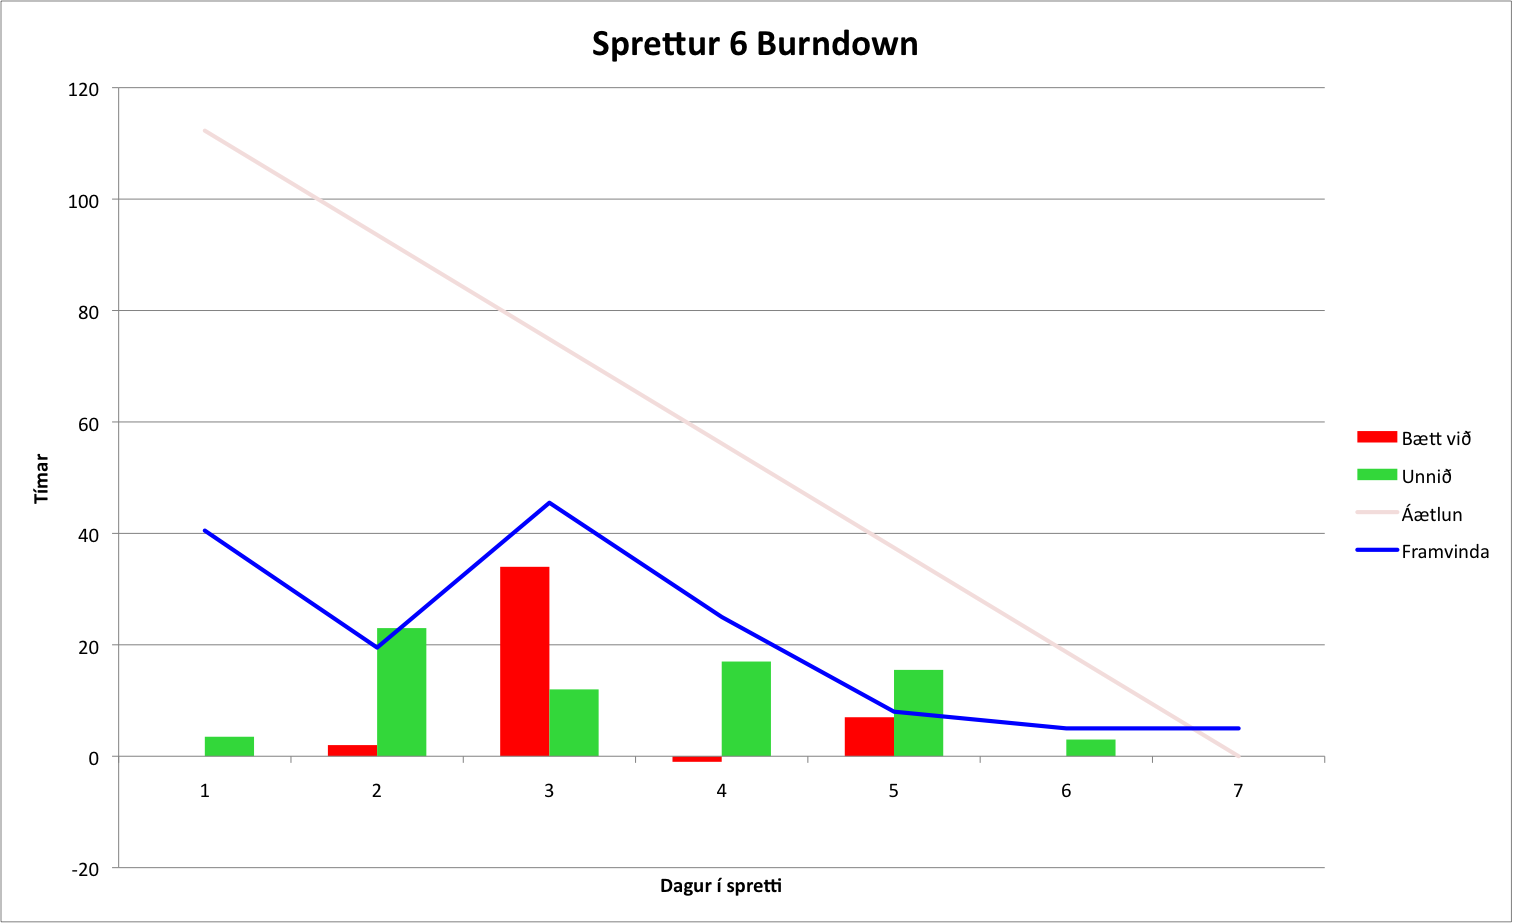
\includegraphics[width=0.72\textwidth]{Sprettur6_Burndown.png}
 \caption{Sprettur 6 Burndown}
\end{figure}

\subsection{Sprettur 7}
Byrjað á lokafrágangi. Allar keyrslustillingar lesnar úr skrá og villumeðhöndlun yfirfarin. Sett upp log kerfi. Álagsprófanir framkvæmdar og 
niðurstöður úr þeim yfirfarnar. Fínstillingar á reikniritum í kjölfar prófanna og villur lagfærðar. 

\begin{figure}[H]
 \centering
 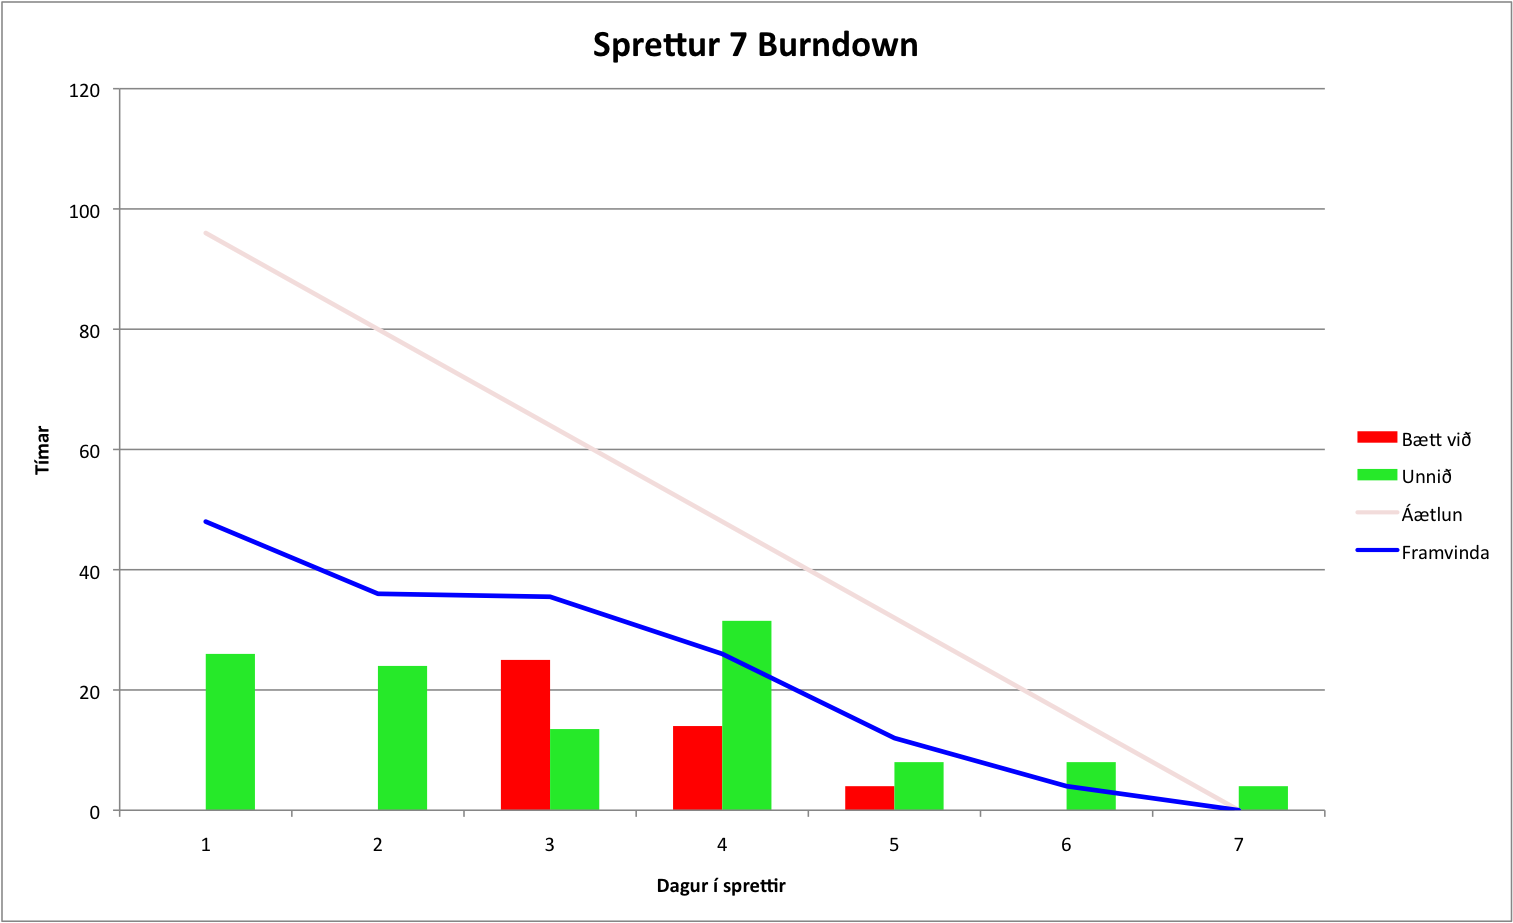
\includegraphics[width=0.72\textwidth]{Sprettur7_Burndown.png}
 \caption{Sprettur 7 Burndown}
\end{figure}

\subsection{Sprettur 8}
Skýrslugerð í aðalatriði í lokasprett. Lokafrágangur á kóða. Læddum inn einni bætingu á reikniaðferðum og prófuðum uppá nýtt.
\begin{figure}[H]
 \centering
 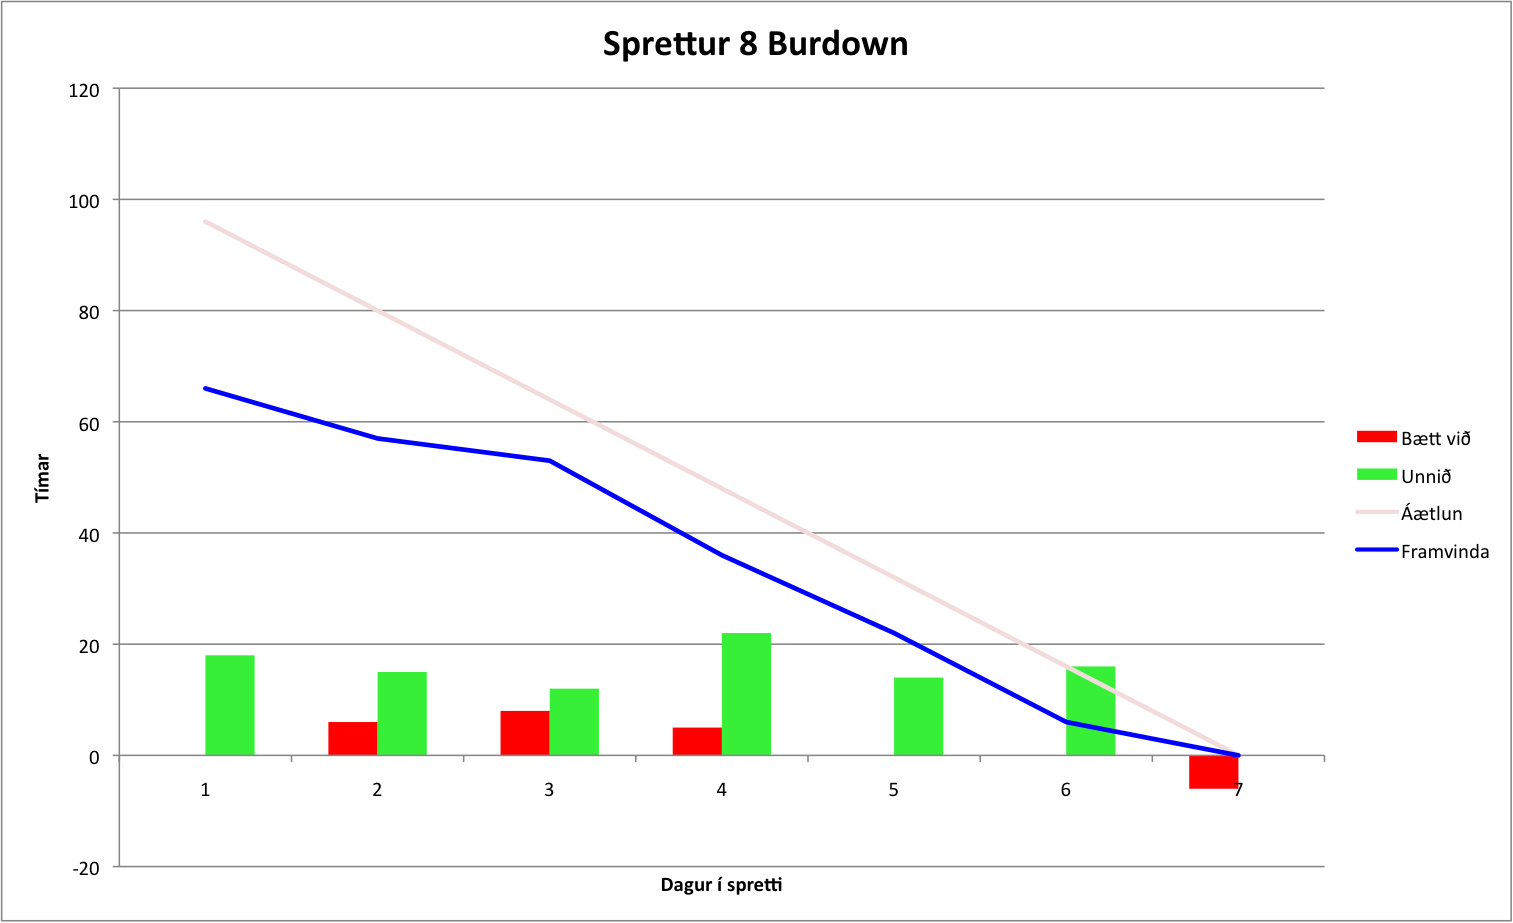
\includegraphics[width=0.72\textwidth]{Sprettur8_Burndown.png}
 \caption{Sprettur 8 Burndown}
\end{figure}



\end{document}